\section{Zadanie 2: Aproksymacja w przestrzeniach unitarnych}
\subsection{Charakterystyka metody i problem}
Celem niniejszego zadania jest ustalenie optymalnej aproksymacji \( h^* \) funkcji \( f \) w przestrzeni unitarnej \( V \), poprzez minimalizację odległości w określonej normie: \[
\|h^* - f\| = \inf \{\|u - f\| : u \in U\},
\] przy założeniu, że \( U \) stanowi podprzestrzeń \( V \). Opierając się na twierdzeniach teorii aproksymacji: 
\begin{itemize}
    \item Rozwiązanie \( h^* \) istnieje i jest unikalne.
    \item Funkcja \( h^* \) jest optymalna, wtedy i tylko wtedy gdy różnica \( f - h^* \) jest ortogonalna do \( U \), tj. \( \langle f - h^*, u \rangle = 0 \) dla każdego \( u \in U \).
    \item Aproksymację \( h^* \) można wyrazić jako kombinację liniową elementów bazy \( U \).
\end{itemize}
\subsection{Metoda rozwiązania}
% TODO tutaj referencje do notatek z wykładu, jak kolwiek to zrobić 
Zakłada się, iż baza \( U \) jest złożona z funkcji \( \{f_i\}_{i \in I} \). Ze względu na właściwość ortogonalności różnicy \( f - h^* \) względem \( U \), zachodzi: \[
\langle f - h^*, f_i \rangle = 0 \quad \text{dla każdego } i \in I.
\] 
W rezultacie uzyskujemy jednoznaczną reprezentację \( h^* \): 
\[
    h^* = \sum_{i \in I} a_i f_i.
\] 
Oznacza to, że współczynniki \( a_i \) aproksymacji \( h^* \) w bazie \( U \) można wyznaczyć, rozwiązując układ równań: 
\[
\langle f, f_i \rangle = \sum_{j \in I} a_j \langle f_j, f_i \rangle.
\] 
w postaci macierzowej $Aa = b$: 
\[
\begin{bmatrix} 
\left<f_1, f_1\right> & \left<f_2, f_1\right> & \cdots & \left<f_n, f_1\right> \\ 
\left<f_1, f_2\right> & \left<f_2, f_2\right> & \cdots & \left<f_n, f_2\right> \\ 
\vdots & \vdots & \ddots & \vdots \\ 
\left<f_1, f_n\right> & \left<f_2, f_n\right> & \cdots & \left<f_n, f_n\right> \\ 
\end{bmatrix} 
\begin{bmatrix} 
a_1 \\ a_2 \\ \vdots \\ a_n \\ 
\end{bmatrix} = 
\begin{bmatrix} 
\left<f, f_1\right> \\ 
\left<f, f_2\right> \\ 
\vdots \\ 
\left<f, f_n\right> \\ 
\end{bmatrix}
\]
\subsection{Przeprowadzane testy} Dla ewaluacji jakości aproksymacji: \begin{itemize}
    \item Porównano błąd aproksymacji w metrykach Chebyshev'a i $L^2$
    \item Sprawdzono zbieżność funkcji aproksymowanych do oryginalnej funkcji dla różnych stopni wielomianów.
\end{itemize} 
\begin{center}
\begin{minipage}{0.92\textwidth}
    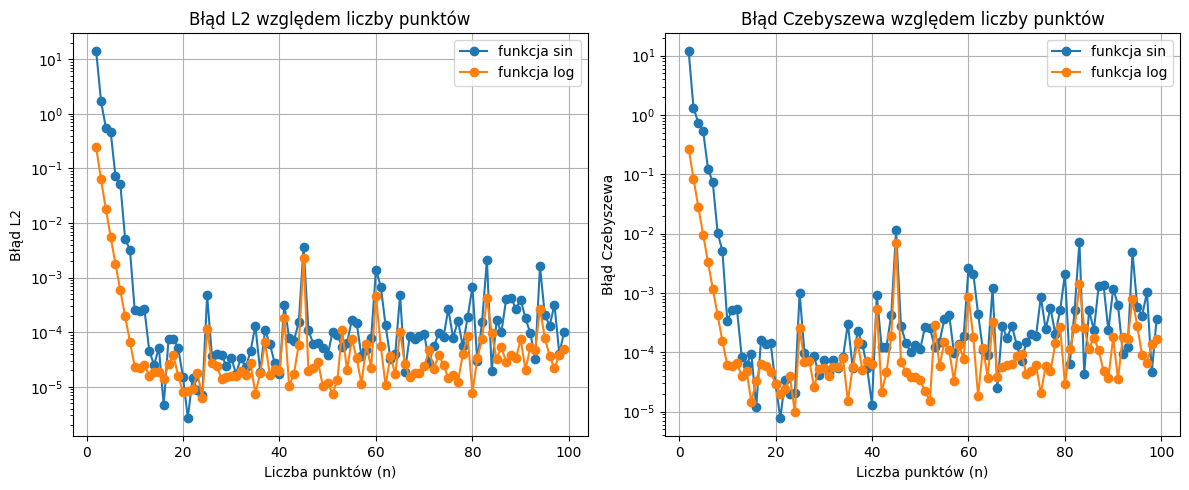
\includegraphics[width=\textwidth]{wykresy/zadanie 2/blad_punkty.png}
\end{minipage}
\hfill
\begin{minipage}{0.45\textwidth}
    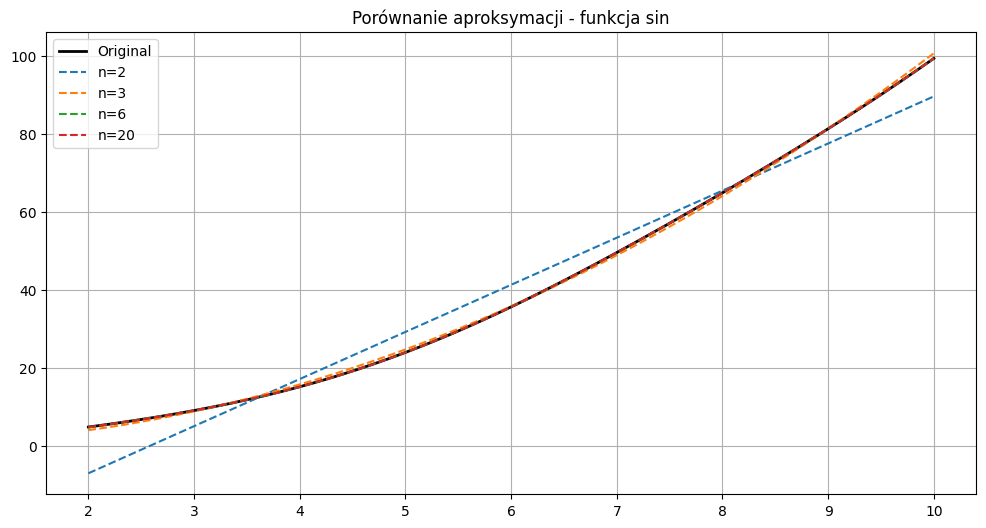
\includegraphics[width=\textwidth]{wykresy/zadanie 2/porownanie_sin.png}
\end{minipage}
\begin{minipage}{0.45\textwidth}
    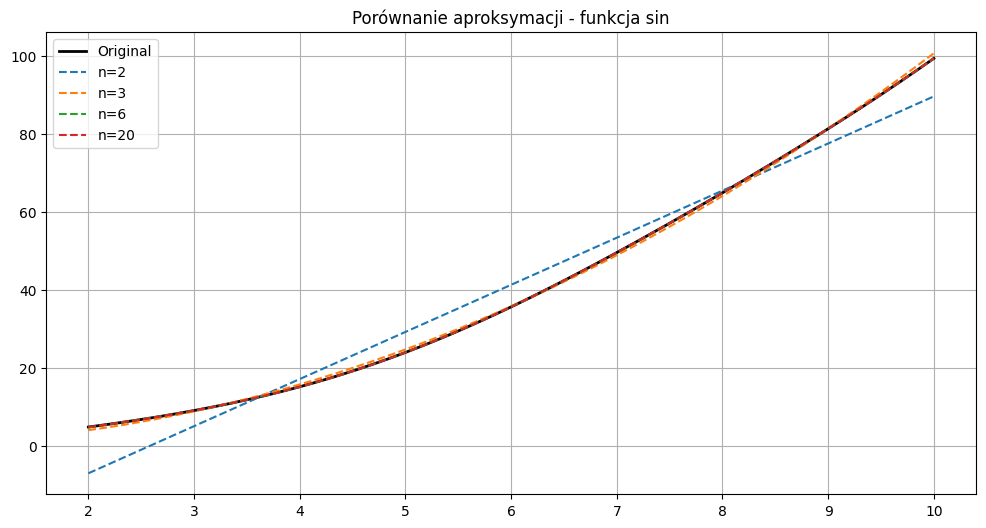
\includegraphics[width=\textwidth]{wykresy/zadanie 2/porownanie_sin.png}
\end{minipage}
\end{center}
\subsection{Wnioski i analiza } 
\begin{itemize}
    \item Metoda minimalizacji odległości \( h^* \) osiąga mniejszy błąd w obu metrykach w porównaniu do metod interpolacji, poprzednio $10^{-1}$ teraz $10^{-4} - 10^{-6}$
    \item Funkcje aproksymowane metodą \( h^* \) szybciej zbliżają się do oryginalnej funkcji, co widać na wykresach porównujących zbieżność, poprzednio koło $25-30$ tutaj $10-20$.
\end{itemize}
\paragraph{Porównanie złożoności obliczeniowej} 
\begin{itemize}
    \item \textbf{Interpolacja Lagrange'a:} \( O(n^2) \).
    \item \textbf{Metoda Newtona:} \( O(n^2) \).
    \item \textbf{Minimalizacja odległości \( h^* \):} \( O(n^3)\), co wynika z potrzeby rozwiązania układu równań metodą $LU$.
\end{itemize}
\paragraph{Wnioski}
\begin{itemize}
    \item Metoda minimalizacji \( h^* \) oferuje lepszą dokładność i szybszą zbieżność w porównaniu z wcześniejszymi.
    \item Dokładność aproksymacji wzrasta wykładniczo ze wzrostem stopnia wielomianu, co pozwala na efektywną aproksymację nawet dla funkcji o skomplikowanej strukturze. 
    % TODO tutaj odnośnik do ref z LAPACK Examples
\end{itemize}